\section{Design, Computation and Further Results of the Finite-Sample Study}
\label{supp:numerical}

\subsection{Design and Objectives}
\label{supp:design}

The study had four objectives. The first was to compare sample CFI, TLI, RMSEA and SRMR with their population values and to determine how often the one-factor model meets conventional cutoffs. The second was to examine the size and direction of loading imbalance, including whether averaging across replications obscures solutions that favor different traits. The third was to assess whether initial values return higher-objective solutions that favor the weaker block. The fourth was to examine these patterns under categorical estimation.

The design crossed 92 populations, four sample sizes (250, 500, 1,000 and 2,000), and three response formats, yielding 1,104 cells. We generated 1,000 replications per continuous cell and 500 per ordinal cell. Ordinal responses had four categories. Symmetric thresholds were $-.8$, 0 and .8; skewed thresholds were .3, 1.0 and 1.7, representing the concentration at low scores often encountered with symptom items. Table~\ref{tab:simulation-design} gives the population conditions.

\begin{table}[t]
\centering\small
\caption{Populations in the finite-sample study. Each population was studied at $N=250$, 500, 1,000 and 2,000, using continuous responses and two four-category response formats. The four objectives are defined in the text.}
\label{tab:simulation-design}
\begin{tabularx}{\textwidth}{@{}>{\raggedright\arraybackslash}p{2.1cm}>{\raggedright\arraybackslash}p{2.3cm}>{\raggedright\arraybackslash}p{2.3cm}LL@{}}
\toprule
Design & Blocks & Loadings & Trait correlations & Purpose \\
\midrule
A. Exchangeable & $m = 4$ or 8 per trait & $\lambda = .5$ or .7 & 0 to .9 in steps of .1, plus $\varphi^*$, $1/p$, $1/(2p)$ and, at $m = 4$ and $\lambda = .5$, .08 & Objectives 1, 2 and 4; ULS arm for Theorem~\ref{thm:uls} \\
B. Unequal loadings & 4 and 4 & .68 and .72; .60 and .80 & 0 to .9 in steps of .1, plus .01, .24 and .409 & Objectives 2 and 3, against Proposition~\ref{prop:unequal} and Figure~\ref{fig:2} \\
C. Unequal lengths & 9 and 7 (PHQ-ADS layout) & .75 for all items & 0 to .9 in steps of .1, plus .653, .865 and .912 & Objectives 1 to 3 for the PHQ-ADS case of Section~\ref{sec:phq} \\
\bottomrule
\end{tabularx}
\end{table}

Each replication was fitted in lavaan (Rosseel, 2012) with a one-factor model and a correlated two-factor model; the two-factor fits are archived and, apart from the convergence summary below, not reported further. Continuous responses were analyzed by ML, with an additional ULS analysis in Design A at $N=500$ and 2,000; ordinal responses were analyzed by WLSMV and by ML applied to the scores 0 to 3. The multistart refits in Designs B and C, at $N=500$ and 2,000, covered the one-factor ML fits to continuous items and to the scores of both ordinal formats. Monte Carlo standard errors are at most .005 for the mean contrasts in Figure~\ref{fig:4}, .003 for mean CFI and .001 for mean RMSEA in Designs A and C, .008 for default-start mean CFI and .0022 for mean RMSEA in Design B, and .016 (1,000 replications) or .022 (500 replications) for proportions.

Loading magnitude and polarity were summarized separately. Let $\bar l_A$ and $\bar l_B$ denote the block means of the standardized loadings, oriented by one common sign such that $m_A\bar l_A+m_B\bar l_B\ge0$. Define the signed contrast $D=\bar l_A-\bar l_B$, the magnitude contrast $M=|\bar l_A|-|\bar l_B|$, and the normalized magnitude contrast
\[
C_{\mathrm{mag}}=\frac{|\bar l_A|/\lambda_A^{\mathrm{ref}}-|\bar l_B|/\lambda_B^{\mathrm{ref}}}{|\bar l_A|/\lambda_A^{\mathrm{ref}}+|\bar l_B|/\lambda_B^{\mathrm{ref}}},
\]
where $\lambda_A^{\mathrm{ref}},\lambda_B^{\mathrm{ref}}>0$ are reference block loadings and the denominator must be positive. The references are the generating loadings for continuous ML, ULS and WLSMV, and the stored population score-scale loadings for ML on scores. We report mean $|C_{\mathrm{mag}}|$, mean $|M|$, and the frequency of opposite block signs. These quantities describe loading patterns; they are not factor-score estimates.

The directional proportions of Section~\ref{sec:numerical}, which count fits with $M>.1$ among those with $|M|>.1$, are conditional on selection and are undefined when no fit is selected. The separate weaker-block flag used in the multistart archive compares reference-normalized magnitudes, $|\bar l_A|/\lambda_A^{\mathrm{ref}}$ and $|\bar l_B|/\lambda_B^{\mathrm{ref}}$, for the population-designated weaker block; it does not use the .1 cutoff.

\subsection{Population Reference Points}

The ML thresholds in Design A were .25 and .20 for loading .5 with $m=4$ and 8, respectively, and .41 and .37 for loading .7. Design B used .41 as an exchangeable reference at the mean loading; unequal loading blocks do not have a symmetric solution. Design C likewise has no symmetric solution because its block lengths differ. The additional low-correlation grid points in Design A were chosen to cover estimator-specific thresholds.

For ULS, the population threshold is $1/p$. WLSMV fits polychoric correlations by weighted least squares, with each correlation weighted by its inverse asymptotic variance. Let $\omega$ be the ratio of cross-block to within-block weights. For $\omega>(m-1)/m$, Proposition~\ref{cor:wls} places the transition at $\varphi_\omega$ in equation~\eqref{eq:wls-threshold}, below which the symmetric solution ceases to be the global minimizer; $\varphi_\omega$ reduces to $1/p$ when $\omega=1$. In the evaluated exchangeable ordinal designs, within-block correlations were estimated more precisely, giving $\omega<1$ and the lower WLSMV thresholds reported in Section~\ref{sec:estimators}. At $m=4$ and loading .5, these were approximately .08: .081 for symmetric categories and .076 for skewed categories. For Design B, the weaker-block minimum exists below the documented folds $\varphi_f=.242$ for loadings .68 and .72, and .017 for loadings .60 and .80.

The second study objective also had an asymptotic motivation. In Gaussian spiked-covariance models with identity noise, as dimension and sample size grow proportionally, a spectral transition occurs at spike excess $\sqrt{p/N}$ (Baik et al., 2005; Paul, 2007). Comparing $\kappa_-$ with this scale provides a heuristic for dependence on $N$ and $\varphi$. It is not a finite-sample detection boundary for the loading contrasts used here.

\subsection{Numerical Conventions and Retained Evidence}

Population continuous-ML references were obtained by multistart fitting, are reported as the best solutions found, and were checked against the closed forms where they apply. Population ML on scores used the exact score covariance matrix. For WLSMV, the DWLS correlation weights were computed numerically from the influence function at the true polychoric correlations and thresholds. The full asymptotic covariance matrix used for the corrections was estimated from 200,000 generated observations, and reference fit indices were evaluated at nominal $N=1{,}000{,}000$. Thus, the WLSMV reference calculation combines analytic population inputs with numerically estimated correction ingredients. We distinguish unscaled WLSMV indices, scaled indices based on scale-and-shift adjusted test statistics, and robust categorical indices based on a normal-theory discrepancy at the DWLS estimates with separate corrections (Savalei, 2021).

All simulation fits, including the multistart refits, were run in R 4.5.1 (R Core Team, 2025) with lavaan 0.6-20 (Rosseel, 2012), the versions recorded in the archived output; the controls in Appendix~\ref{supp:controls} used R 4.6.1 and lavaan 0.7-2. The simulation required approximately 150 CPU hours for 2.3 million fits (one-factor and two-factor fits; ULS was fitted with the one-factor model only; the multistart refits in Designs B and C are additional). One seed per population and sample size was shared by the three response formats: the cell seed was $100{,}000\,k+10{,}000\,j$ for population $k$ and the $j$th sample size ($j=1,\dots,4$ for $N=250$, 500, 1,000 and 2,000), and replication $r$ used the cell seed plus $r$. No replication returned an error. All 1.21 million one-factor fits reported convergence; among the 1.10 million two-factor fits, nonconvergence was at most 0.2\% (1 of 500) in any cell, and 33 had a negative estimated uniqueness. Of the one-factor fits, seven had negative estimated uniquenesses: six ML fits to ordinal scores and one WLSMV fit. These unconstrained negative estimates are outside the zero-uniqueness ML boundary classification. The archived summaries retain them and also give the subset with positive recorded uniquenesses. None occurs in the $N=2{,}000$ subsets used in Figures~\ref{fig:4} and \ref{fig:5}.

For multistart fitting in Designs B and C, the factor variance was fixed at 1 (\texttt{std.lv = TRUE}). Each fit used the two default item orders and 20 random starts, with loadings sampled uniformly on $(0,1)$ and uniquenesses uniformly on $(.2,1)$. Reported-converged solutions were grouped at standardized-loading tolerance .002. The lowest objective in each group was retained, and groups were compared at tolerance $10^{-7}$ in lavaan's objective. The archive does not retain the objective from every individual start. A positive recorded uniqueness, reported convergence, or agreement with the lowest observed objective does not establish stationarity or global optimality.

For Table~\ref{tab:4}, default and best-found fits were paired within replication. For ML, lavaan's objective is $\mathit{fx}=F/2$. The estimated baseline noncentrality was reconstructed as
\[
B=\frac{T-\mathit{df}}{1-\mathrm{CFI}_{\mathrm{default}}},
\qquad T=2N\,\mathit{fx}.
\]
Best-found CFI used $T_{\mathrm{best}}=2N\,\mathit{fx}_{\mathrm{best}}$ and the standard nonnegative truncations,
\[
\mathrm{CFI}_{\mathrm{best}}
=1-\frac{\max(T_{\mathrm{best}}-\mathit{df},0)}
{\max(T_{\mathrm{best}}-\mathit{df},B,0)}.
\]
The inversion domain was satisfied by all 18,000 pairs. The accompanying evidence contains the paired terms, selected fit rows, figure exports and calculation scripts. The population calculations are also implemented in the accompanying R package \texttt{undeRfactor} (version 0.2.0, \url{https://github.com/atomashevic/undeRfactor}).

\subsection{Further Results on Fit Indices}
\label{supp:fit}

The agreement between sample fit indices and their population references depended on the solution returned. In Designs B and C, mean CFI at the best solution found differed from its population value by at most .004 at $N=500$ and .0013 at $N=2{,}000$; the corresponding differences for RMSEA were .0023 and .0006. In Design A with four items per trait and loading .5 (default starts), mean CFI exceeded its population value by about .05 throughout $\varphi\le\varphi^*$ at $N=250$ (maximum .056). At $N=1{,}000$ and 2,000 the bias peaked at $\varphi=.2$, just below $\varphi^*=.25$ (.019 and .016). This peak near the threshold at the larger sample sizes is consistent with the small curvature in the direction that differentiates the blocks. Because these population CFI values are below .62, the bias does not affect cutoff decisions in this range. RMSEA remained within .003 of its population value at $N\ge1{,}000$. At $N=250$, the upward bias of SRMR reached .03. The sample and population half-pass correlations compared in Section~\ref{sec:numerical} were both located by linear interpolation between evaluated correlations, which are spaced .1 apart outside the added points. The cutoff-passing comparison at $\varphi=.912$ reported there used skewed four-category items for WLSMV (Figure~\ref{fig:3}).

The robust WLSMV comparison in Section~\ref{sec:numerical} covers the evaluated populations with $\varphi\ge.7$, which included every evaluated population meeting continuous-ML CFI $\ge.95$. At lower correlations, robust CFI could be lower, and WLSMV could retain a composite solution where ML produced unequal block loadings.

Unscaled and scaled WLSMV indices were more lenient in the near-cutoff comparisons. Figure~\ref{fig:3} shows the PHQ-ADS layout with skewed four-category items at $N=250$. At INCPAD's correlation, unscaled WLSMV CFI met .95 in 92\% of samples and scaled CFI did so in 1\%; neither continuous ML nor robust WLSMV CFI met the cutoff. At ESCAPE's correlation of .865, CFI and RMSEA often gave different decisions. CFI passed in 57\% of continuous-ML samples and 42\% of robust WLSMV samples, whereas RMSEA passed in 26\% and 21\%, respectively; scaled CFI passed in 99\%. Section~\ref{sec:numerical} reports the comparison at SCOPE's correlation of .912.

\begin{figure}[t]
\centering
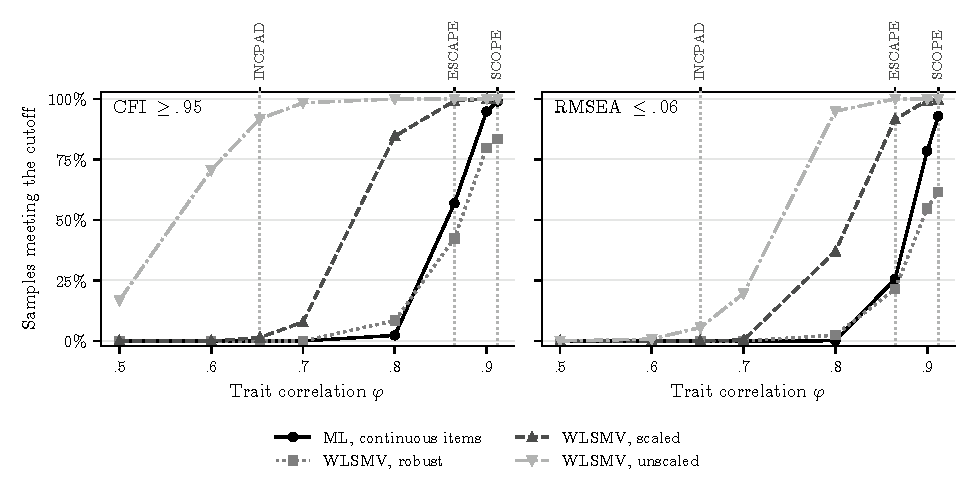
\includegraphics[width=\textwidth]{fig3.pdf}
\caption{Share of samples in which the one-factor model meets CFI $\ge .95$ (left) and RMSEA $\le .06$ (right) in the PHQ-ADS layout: 9 and 7 items with loading .75, $N = 250$. ML on continuous items, and lavaan's robust, scaled and unscaled WLSMV indices on skewed four-category items. Vertical lines mark the trait correlations of the three trials. Each point is based on 1,000 (ML) or 500 (WLSMV) replications; lines join the evaluated correlations.}
\label{fig:3}
\end{figure}

\subsection{Further Results on Loading Imbalance and Item Order}
\label{supp:imbalance}

In the setting of Figure~\ref{fig:4}, mean $|C_{\mathrm{mag}}|$ under ML was .500 at $\varphi=.2$. Under ULS, it was .834 at 0, .317 at its population threshold $1/p=.125$, .117 at .2 and .050 at .3; under WLSMV on symmetric categories, it was .037 at .2.

The unnormalized magnitude contrast showed both close agreement with the population result and attenuation at smaller sample sizes. With four items per trait, loading .7 and $N=2{,}000$, mean $|M|$ under ML at $\varphi=.2$ was .458, compared with .459 in the population. With four items per trait, loading .5 and $N=250$, it was .412 at $\varphi=0$, compared with .50 in the population. These continuous summaries describe the amount of imbalance without treating a reference distribution at one correlation as a test at another.

The effect of averaging depended on both estimator and sign convention. For continuous ML at $\varphi=0$, with four items per trait, loading .7 and $N=2{,}000$, mean $D$ and mean $|D|$ were both .701 after common sign orientation, while mean $|M|$ was .674. Opposite block signs occurred in 510 of the 1,000 fits, so the signed and magnitude contrasts cannot be interchanged. Under ULS, averaging did obscure imbalance: at its population threshold, the mean signed difference was .02 and the mean absolute difference was .30.

Among Design A fits selected by $|M|>.1$, 86\% of continuous-ML fits favored the first-listed block at $N=2{,}000$, compared with 74\% at $N=250$. The first-block/selected counts behind the directional proportions at $N=2{,}000$ in Section~\ref{sec:numerical} were 24,767/28,719 (continuous ML), 11,508/13,501 (ML on scores), 12,385/18,344 (ULS) and 2,649/4,746 (WLSMV). Each ratio pools 53 population cells, and the ordinal analyses used symmetric categories.

With the weaker block listed first, continuous ML returned a higher-objective group favoring that block in 27 to 45\% of samples with loadings .60 and .80 at $\varphi\le.01$, for $N=500$ and 2,000, compared with 94 to 100\% for loadings .68 and .72 at $\varphi\le.1$. With loadings .68 and .72, $\varphi=0$ and $N=2{,}000$, the default fit gave CFI $=.44$ and RMSEA $=.250$, compared with .56 and .223 at the best solution found, and the default factor favored the trait with lower generating loadings. Listing the weaker block last produced no weaker-block flags in any of the 234 archived cell--analysis combinations (78 population--sample-size cells $\times$ three ML analyses). Because none of the 761 replications that retained a higher-objective group under the weaker-last order had a weaker-block flag, a higher objective and a weaker-block loading pattern are distinct properties. With loadings .68 and .72 at $\varphi=.3$, above the population fold, higher-objective weaker-block groups occurred in 26\% of default fits at $N=500$ and 7\% at $N=2{,}000$. Across cells, the largest mean recorded fraction of converged random starts assigned to the selected higher-objective weaker-block group was 36\%, in a cell analyzed by ML on ordinal scores (35.5\% for continuous ML).

\subsection{Starting Covariance and Identification Controls}
\label{supp:controls}

Equal starting covariances did not imply equal optimization paths. Six population cases were refitted under two item orders and two identifications, using default starts and a common starting covariance (R 4.6.1, lavaan 0.7-2). The 48 fits included 47 reported convergences. Gradient and Hessian checks supported 39 strict local minima and identified two saddles; seven fits exceeded the gradient tolerance of $10^{-6}$. Evidence for a strict local minimum additionally required a smallest Hessian eigenvalue above $10^{-5}$.

The common starting covariance used loadings .6 and uniquenesses .64 under unit latent variance. In the unequal-loading cases, all 20 common-start fits agreed with the best numerical reference objective within $3.8\times10^{-11}$. Four exceeded the gradient tolerance, including one nonconverged fit, so objective agreement did not verify every fit as a minimum. In the exchangeable case with loading .7 and $\varphi=.3$, unit-variance identification reached the symmetric saddle, with $F=.970752$ and smallest Hessian eigenvalue $-.306480$. Marker identification reached either analytic global minimum, with $F=.940795$, depending on item order.

\subsection{Assessment of the Study Predictions}

Four predictions were stated with the design, and a fifth was added after the pilot from the categorical weighted-least-squares result. The first predicted that mean CFI and RMSEA for continuous ML would be within .01 of their population values at $N\ge1{,}000$. For Designs B and C at the best solution found, and for Design A at the default solution, RMSEA met this prediction in every evaluated cell. CFI did so except in Design A with loading .5 near $\varphi^*$, where the default-start difference reached .019 at $N=1{,}000$. Higher-objective default solutions below the fold lowered CFI by as much as .23.

The second prediction was that exchangeable designs would favor the two blocks about equally often, causing mean loadings to resemble a composite. The directional summaries did not support equal selection under the default ML start: conditional first-block proportions at $N=2{,}000$ were 86\% for ML, 85\% for ML on scores, 68\% for ULS and 56\% for WLSMV. The ordinal summaries used symmetric categories and selection required $|M|>.1$.

The third prediction was that unequal-loading designs would favor the stronger block and that weaker-block minima would occur essentially below $\varphi_f$. The best solutions found supported the stronger-block prediction. Higher-objective groups favoring the weaker block also occurred above the population fold, but these retained sample groups do not certify local minima.

The fourth prediction placed the ULS transition at $1/p$, below the ML threshold. Sample imbalance decreased across this point without disappearing. At $N=2{,}000$, mean $|C_{\mathrm{mag}}|$ was .117 at $\varphi=.2$ and .050 at .3 for ULS, compared with .500 and .312 for ML. The fifth prediction related WLSMV imbalance to its own population threshold. With four items per trait and loading .7, the population solution remained a composite; sample mean $|C_{\mathrm{mag}}|$ was .102 at $\varphi=0$ and .037 at .2 for symmetric categories and $N=2{,}000$. The diagnostics describe magnitude and polarity separately and do not define a false-positive rate by calibration at another correlation.
